\documentclass[10pt]{article}

\usepackage{graphicx} % Required for inserting images
\usepackage[margin=0.75in]{geometry} 
\usepackage{amsmath,amsthm,amssymb,amsfonts, enumitem, fancyhdr, color, comment, graphicx, environ}
\usepackage{cases}
\usepackage{subcaption}
\usepackage{xcolor}
\usepackage{MnSymbol} 
\usepackage{float}
\usepackage[boxruled,vlined,noline,]{algorithm2e}

\RequirePackage[colorlinks,citecolor=blue,urlcolor=blue,hypertexnames=true]{hyperref}
\usepackage{tikz}
\usetikzlibrary{arrows.meta}
\usetikzlibrary{arrows}
\usetikzlibrary{shapes.multipart}
\usetikzlibrary{positioning, fit} 

\pagestyle{plain}
\geometry{top=75pt, bottom=75pt, left=45pt, right=45pt}


\DeclareMathOperator*{\argmax}{arg\,max}
\DeclareMathOperator*{\argmin}{arg\,min}
\DeclareMathOperator*{\pperp}{\perp \!\!\! \perp}

\newtheorem{ass}{Assumption}
\newtheorem{thm}{Theorem}
\newtheorem{cor}{Corollary}
\newtheorem{lem}{Lemma}
\newtheorem{cond}{Condition}
\newtheorem{mydef}{Definition}
\theoremstyle{remark} \newtheorem{rem}{Remark}





\title{Policy learning for Proximal Quantile-Optimal DTR}
\author{CTL}
\date{}

\begin{document}
\maketitle
\section{Setup}
\subsection{Problems}
Consider a problem of $K(K\geq1)$ stage dynamic treatment regimes estimation by maximizing quantile value with time-varying unmeasured confounders under the proximal causal inference framework.

\subsection{Notations}
\begin{itemize}
    \item $Y_k$: outcome variables
        \begin{itemize}
            \item $k=0$: the baseline measurement of the outcome
            \item $k=1,\ldots,K-1$: the intermediate outcome
            \item $k=K$: the ultimate outcome
        \end{itemize}
    \item $A_k$: dichotomous treatment variables satisfy $A_k \in \mathcal{A}_k=\mathcal{A}_k, \, \forall k=1,2,\ldots,K$
    \item $U_k$: time-varying unmeasured confounders, $k=0,1,\ldots,K-1$
    \item $Z_k$: treatment-inducing proxies, $k=1,2,\ldots,K$
    \item $W_k$: outcome-inducing proxies, $k=1,2,\ldots,K$
    \item $\bar{X}_k$: the sequence from the initial stage to $k$th stage of variable $X$
    \item $\mathcal{D}_k$: the class of candidate regimes at $k$th stage, and $\mathcal{D} =\{\mathcal{D}_1,\ldots, \mathcal{D}_K\}$ denotes the set of all candidate regime sequences
    \item $d_k$: the regime function $d_k=d_k(\bar{Y}_{k-1},\bar{a}_{k-1})$, where $d_k \in \mathcal{D}_k$ 
    \textcolor{blue}{\begin{rem}: $\bar{Y}_{k-1}$ also depends on $\bar{a}_{k-1}$, thus $d_k$ can also be written as $d_k=d_k(\bar{Y}_{k-1}(\bar{a}_{k-1}),\bar{a}_{k-1})$\end{rem}}
\end{itemize}

\subsection{Identification Framework}
\begin{itemize}
    \item Potential outcomes for $K$ stages: define $Y_k(\bar{d}_k)$ as the intermediate potential outcomes at (until) stage $k$. Then the ultimate potential outcomes $Y_{K}(\bar{d}_K)$ that would be achieved under regime $\bar{d}_K=(d_1,d_2,\ldots,d_K)$ are collected through the sequence
    \[
    \{Y_0, Y_1(d_1),Y_2(\bar{d}_2),\ldots,Y_{K-1}(\bar{d}_{K-1}),Y_K(d_K)\},
    \]
    where we define
    \[
    Y_k(\bar{d}_k) = \sum_{\bar{a}_k}[Y_k(\bar{a}_k)\prod_{j=1}^k I(d_j(\bar{Y}_{j-1}(\bar{a}_{j-1}),\bar{a}_{j-1}) = a_j)], \quad k=1,2,\ldots,K.
    \]
    \item Value function: the value function for regime $\bar{d}_K$ defined as 
    \[
    V(\bar{d}_K) = \mathbb{E}[Y_K(\bar{d}_K)]
    \]
    \item Quantile-value function: similar to the value function, we denote the quantile-value function as 
    \[
    QV(\tau,\bar{d}_K) = Q_{\tau}[Y_K(\bar{d}_K)],
    \]
    where $\tau \in (0,1)$ and $Q_{\tau}(\bar{d}_K)$ denotes the $\tau$th quantile of $\bar{d}_K$. Specifically, $Q_\tau[Y_K(\bar{d}_K)] = \inf \{t: F_d(\cdot)>\tau\}$, where $F_d$ is the distribution function of $Y_K(\bar{d}_K)$.
    \item Goal: find the quantile-optimal regimes $d^*=\bar{d}_K^*$ that maximize the quantile-value function
    \[
    d^* = \bar{d}_K^*= \argmax_{d\in\mathcal{D}} Q_\tau[Y_K(\bar{d}_K)].
    \]
    \item Characterization of $\tau$th quantile: for a given treatment regime$d=\bar{d}_K$, an estimation of quantile-value is 
    \[\begin{aligned}
    QV(\tau,\bar{d}_K) &= \argmin_{q} \mathbb{E}[\rho_{\tau}(Y_K(\bar d_K)-q)] \\
    &= \argmin_{q} \sum\limits_{\bar y_K}\sum\limits_{\bar a_K}[\rho_{\tau}(y_K-q)\prod_{j=1}^K I\left(d_j(\bar y_{j-1}, \bar a_{j-1})=a_j\right)f(\bar Y_K(\bar a_K)=\bar y_K)],
    \end{aligned}\]
    where $\rho_\tau(u) := u(\tau-I\left(u<0\right))$ is the check function (quantile loss).
    
    Then we can characterize the quantile-optimal DTR as 
    \[\begin{aligned}
        d^* = \argmax_{d\in \mathcal{D}}\biggl\{ \argmin_{q} \sum\limits_{\bar y_K}\sum\limits_{\bar a_K}[\rho_{\tau}(y_K-q) 
        \prod_{j=1}^K I\left(d_j(\bar y_{j-1}, \bar a_{j-1})=a_j\right)
        f(\bar Y_K(\bar a_K)=\bar y_K \mid Y_0=y_0) f(Y_0=y_0)]  \biggr\}.
    \end{aligned}\]
    Thus, it is critical to identify the conditional joint density of the potential outcomes:
    \[f(\bar Y_K(\bar a_K)=\bar y_K \mid Y_0=y_0).\]
\end{itemize}



\section{Proximal Identification via treatment bridge function}
\subsection{Proximal framework}
A causal Directed Acyclic Graph (DAG) that describes a 2-stage longitudinal proximal causal inference framework is shown in Figure \ref{fig: 2SDTR}. 
Simply put, because of the existence of unmeasured confounding U, we need to find a suitable set of instrumental variables W and Z to reflect the information of U, thereby helping to identify.
We now have the following identifiability assumptions for the proximal setting.
\begin{figure}[htb]
    \centering
    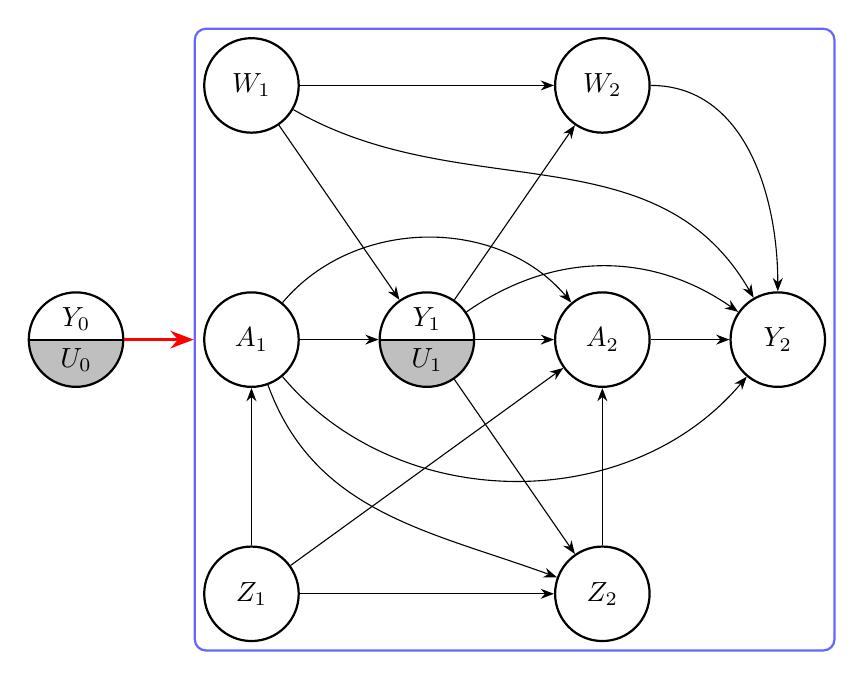
\begin{tikzpicture}[
        node distance=1cm,
        thick,
        % 
        normal node/.style={
            circle,
            draw,
            minimum size=1.2cm,
            font=\sffamily\bfseries,
            align=center,
        },
        % 
        split node/.style={
            circle split,
            draw,
            minimum size=1.2cm,
            inner sep=0.1cm,
            font=\sffamily\bfseries,
            path picture={
                \fill[gray!50] (path picture bounding box.south west) rectangle 
                (path picture bounding box.east |- path picture bounding box.center);
            }
        },
        normal edge/.style={->, >=Stealth, thin},
        highlight edge/.style={->, >=Stealth, very thick, red}
        ]
        
        % Vertices
        
        \node[split node] (Y0-U0) {$Y_0$ \nodepart{lower} $U_0$};
        \node[normal node, right=of Y0-U0] (A1) {$A_1$};
        \node[normal node, above =2cm of A1] (W1) {$W_1$};
        \node[normal node, below =2cm of A1] (Z1) {$Z_1$};
        \node[split node, right=of A1] (Y1-U1) {$Y_1$ \nodepart{lower} $U_1$};
        \node[normal node, right=of Y1-U1] (A2) {$A_2$};
        \node[normal node, above=2cm of A2] (W2) {$W_2$};
        \node[normal node, right=of A2] (Y2) {$Y_2$};
        \node[normal node, below=2cm of A2] (Z2) {$Z_2$};
        
        % Edges
        
        
        \draw[normal edge] (Z1) to (A1);
        \draw[normal edge] (Z1) to (A2);
        \draw[normal edge] (Z1) to (Z2);
        %				
        \draw[normal edge] (A1) to[out=50,in=130] (A2);
        \draw[normal edge] (A1) to[out=310,in=230] (Y2);
        \draw[normal edge] (A1) to[out=290,in=160] (Z2);
        %				
        \draw[normal edge] (W1) to (Y1-U1);
        \draw[normal edge] (W1) to[out=330,in=120] (Y2);
        \draw[normal edge] (W1) to (W2);
        
        \draw[normal edge] (Y1-U1) to[out=35,in=145] (Y2);
        \draw[normal edge] (Y1-U1) to (Z2);
        \draw[normal edge] (Y1-U1) to (W2);
        
        \draw[normal edge] (Z2) to (A2);
        
        \draw[normal edge] (W2) to[out=0,in=90] (Y2);
        
        % 		
        \draw[normal edge] (A1) to (Y1-U1);
        \draw[normal edge] (Y1-U1) to (A2);
        \draw[normal edge] (A2) to (Y2);
        
        \node[draw=blue!60,thick,rounded corners,fit=(A1)(W1)(Z1)(Y1-U1)(A2)(W2)(Z2)(Y2),inner sep=3pt] (sub) {};
        
        \draw[highlight edge] (Y0-U0) to[out=0,in=180] (sub.west);
        % 		
    \end{tikzpicture}
    \caption{A DAG for the $2$-stage longitudinal proximal causal inference framework that satisfies Assumptions 11-13.} 
    \label{fig: 2SDTR}
\end{figure}


\subsection{Identifiability Assumptions}
\begin{ass}[Sequential consistency]
    $Y_k = Y_k(\bar A_k)$ for $k=1,2,\ldots,K$ almost surely.
    \label{ass10}
\end{ass}

\begin{ass}[Treatment-inducing confounding proxies]
    $Y_k(\bar a_k, \bar z_k) = Y_k(\bar a_k)$ for $k=1,2,\ldots,K$ almost surely
    $\Longleftrightarrow Y_k \pperp \bar Z_k \mid (\bar U_{k-1}, \bar Y_{k-1})$.
    \label{ass12}
\end{ass}

\begin{ass}[Sequential proximal latent randomization]
    $\{Y_k(\bar a_k), Y_{k+1}(\bar a_{k+1}), \ldots, Y_K(\bar a_K), \bar W_k\} \pperp \{A_k,\bar Z_k\}|(\bar U_{k-1}, \bar Y_{k-1}, \bar A_{k-1}=\bar a_{k-1})$ for $k=1,2,\ldots,K$ and $a_k \in \mathcal{A}_k$.
    \label{ass13}
\end{ass}

\begin{ass}[Sequential positivity]
    $0< f(A_k=a_k \mid \bar U_{k-1}, \bar Y_{k-1}, \bar A_{k-1}) < 1$ for $k=1,2,\ldots,K$ and $\forall a_k \in \mathcal{A}_k$.
    \label{ass14}
\end{ass}

\begin{ass}[Z-Completeness]
    For a fixed $k$ and $m=K,K-1,\ldots,k+1$, for any square integrable function $g_m(\bar U_{m-1})$ and $\forall \bar y_{m-1}, \bar a_m$,
    \[
    \mathbb{E}[g_m(\bar U_{m-1}) \mid \bar Z_m, \bar a_m, \bar y_{m-1}]=0, \,a.s. \Longleftrightarrow g_m(\bar U_{m-1}) = 0, \, a.s. .
    \]
    \label{ass15}
\end{ass}

\begin{ass}[W-Completeness]
    For a fixed $k$ and $n=1,2,\ldots,k$, for any square integrable function $g_n(\bar U_{n-1})$ and $\forall \bar y_{n-1}, \bar a_n$,
    \[
    \mathbb{E}[g_n(\bar U_{n-1}) \mid \bar W_n, \bar a_n, \bar y_{n-1}]=0, \,a.s. \Longleftrightarrow g_n(\bar U_{n-1}) = 0, \, a.s. .
    \]
    \label{ass16}
\end{ass}

\begin{ass}[Treatment confounding bridge functions]
    For a fixed $k$ and $n=1,2,\ldots,k$, there exist treatment confounding bridge functions $q_{nn}(\cdot)$ such that
    \begin{numcases}{}
        \frac{1}{f(a_1 \mid w_1,y_0)} = \sum_{z_1}q_{11}(z_1,y_0,a_1)f(z_1 \mid a_1,w_1,y_0), & $n=1$ \label{tbf1}\\
        \frac{\sum\limits_{\bar z_{n-1}} q_{n-1,n-1}(\bar z_{n-1}, \bar y_{n-2}, \bar a_{n-1})f(\bar z_{n-1} \mid \bar a_{n-1}, \bar w_n, \bar y_{n-1})}{f(a_n \mid \bar a_{n-1}, \bar w_n, \bar y_{n-1})} = \sum_{\bar z_n}q_{nn}(\bar z_{n}, \bar y_{n-1}, \bar a_{n})f(\bar z_n \mid \bar a_n, \bar w_n, \bar y_{n-1}), & $n=2,\ldots,k$. \label{tbf2}
    \end{numcases}
    \label{ass18}
\end{ass}


\subsection{Identification and estimation}
We first give an identification expression for $K$ stage.
\begin{thm}
    Suppose assumptions \ref{ass10}-\ref{ass18} holds. Then we have
    \begin{equation}
        f(\bar Y_k(\bar a_K)=\bar y_K \mid Y_0=y_0) = \sum_{\bar z_K} q_{KK}(\bar z_K, 
        \bar y_{K-1}, \bar a_K)f(\bar z_K, \bar y_K, \bar a_K \mid y_0)。
    \end{equation}
\end{thm}

Now, for further testing and experimentation, we only consider the situation when $K=2$.
It is natural to obtain an estimate of the target, i.e., the quantile-value function, from the observed data.
\begin{align}
    &\hat{QV}(\tau,\bar d_K) \notag \\
    =& \argmin_{q}  \mathbb{P}_n \bigl\{\rho_\tau(Y_{2}-q)\cdot \hat q_{22}(\bar Z_{2}, \bar Y_{1}, \bar A_{2}) I(d_1(Y_{0})=A_1)I(d_2(\bar Y_{1},A_1)=A_2) \bigr\} \notag \\
    =& \argmin_{q} \frac{1}{n}\sum_{i=1}^n  \bigl\{\rho_\tau(Y_{2,i} - q)\cdot \hat q_{22}(\bar Z_{2,i}, \bar Y_{1,i}, \bar A_{2,i}) I(d_1(Y_{0,i})=A_{1,i})I(d_2(\bar Y_{1,i},A_{1,i})=A_{2,i}) \bigr\}.
    \label{est}
\end{align}



\section{Policy Learning}
Now that we have already derived how to use the treatment bridge function to estimate quantile-value function from\eqref{est}, the next step is to learn the quantile-optimal regimes (policies) $\bar d_2^* = (d_1^*, d_2^*)$ in the policy space $\mathcal{D}$ that maximize the quantile-value function, which can be identified as
\begin{align}
    \bar d_2^* = (d_1^*, d_2^*) =&  \argmax_{(d_1,d_2) \in \mathcal{D}} Q_\tau(Y_2(d_1, d_2))    \notag\\
     =& \argmax_{(d_1,d_2) \in \mathcal{D}} \Big\{\argmin_{q}\mathbb{E} \bigl[\rho_\tau(Y_{2}-q)\cdot q_{22}(\bar Z_{2}, \bar Y_{1}, \bar A_{2}) I(d_1(Y_{0})=A_1)I(d_2(\bar Y_{1},A_1)=A_2) \bigr]\Big\}.  \label{ident}
\end{align}
Solving the quantile-optimal treatment regime $(d_1^*,d_2^*)$ can be deemed as a bi-level optimization with the following two-level optimization:
\begin{itemize}
    \item Inner level optimization: for a fixed $d=(d_1,d_2)$, first solve the quantile-value function to find the optimal quantile:
    \begin{align}
    & Q_\tau(Y_2(d_1,d_2)) = \argmin\limits_{q} \mathbb{E}\big[\rho_\tau(Y_{2}(d_1,d_2) - q) \big] \label{inner}
    \end{align}
    \item Outer level optimization: fixing $Q_\tau(Y_2(d_1,d_2))$, then find the quantile-optimal treatment regimes  
    \begin{align}
    d^* = (d_1^*,d_2^*) = \argmax \limits_{(d_1,d_2)} Q_\tau(Y_2(d_1,d_2)).
    \label{outer}
    \end{align}
\end{itemize}

For the inner level optimization in \eqref{inner}, the quantile-value function can be identified via PIPW \eqref{est} by 
\begin{align}
    &Q_\tau(Y_2(d_1,d_2)) = \argmin_{q}\mathbb{E} \bigl\{\rho_\tau(Y_{2}-q)\cdot q_{22}(\bar Z_{2}, \bar Y_{1}, \bar A_{2}) I(d_1(Y_{0})=A_1)I(d_2(\bar Y_{1},A_1)=A_2) \bigr\} \notag\\
    \Longleftrightarrow \quad & \mathbb{E}\big[I\{Y_2 > Q_\tau(Y_2(d_1,d_2))\}\cdot q_{22}(\bar Z_{2}, \bar Y_{1}, \bar A_{2}) I(d_1(Y_{0})=A_1)I(d_2(\bar Y_{1},A_1)=A_2) \big]= 1-\tau. \label{ilo1}
\end{align}
The above derivation indicates that if we find the optimal quantile value $q^*$ that satisfies the equation \eqref{ilo1} under the fixed regimes $d_1,d_2$, i.e., 
\begin{align}
    \mathbb{E}\big[I\{Y_2 > q^*\}\cdot q_{22}(\bar Z_{2}, \bar Y_{1}, \bar A_{2}) I(d_1(Y_{0})=A_1)I(d_2(\bar Y_{1},A_1)=A_2) \big]= 1-\tau, \label{ilo2}
\end{align}
the optimal $q^*$ can be regarded as a function of polices $d_1,d_2$.
In other words, equation \eqref{ilo2} establishs an implicit function of $q^*$ and $d_1,d_2$,
which allows us to consider $q^*$ as a function of $d_1,d_2$, denoted as $q^*(d_1,d_2)$.

Consequently, the outer level optimization can be simplified as solving
\begin{align}
    (d_1^{*},d_2^{*}) = \argmax_{(d_1,d_2)\in\mathcal{D}}q^*(d_1,d_2). \notag
\end{align}
Furthermore, we consider $q$ as a parameter since our goal is only to find the optimal $d_1,d_2$. 
Denote the survival value function as
$$
SV(d_1,d_2;q) = \mathbb{E} \big[I(Y_2 > q)\cdot q_{22}(\bar Z_{2}, \bar Y_{1}, \bar A_{2}) \cdot  I(d_1(Y_0)=A_1)I(d_2(\bar Y_1, A_1)=A_2) \big].
$$
The goal of outer level optimization can be expressed as 
\begin{align}
    (d_1^{*},d_2^{*}) = \argmax_{(d_1,d_2)\in\mathcal{D}} SV(d_1,d_2;q^*).
\end{align}

In practice, we plan our policy learning in the following steps.
First, we need to pre-estimate the nuisance function $\hat q_{22}(\bar Z_2,\bar Y_1, \bar A_2)$.
Then, we alternately solve the inner level optimization and outer level optimization by an iterative process.


\subsection{Pre-estimation of the treatment bridge function}
Before estimating the policies, we first need to estimate the nuisance treatment bridge function $q_{22}(\bar Z_{2}, \bar Y_{1}, \bar A_{2})$, which also requires the estimation of $q_{11}$ according to assumption \ref{ass18}.
Our method involves using neural networks to estimate the treatment bridge functions, which builds on the idea of the DeepMMR method proposed by (Zhang2025).
Furthermore, we extended their method to a two-stage setting for estimating the treatment bridge function $q_{22}(\bar Z_{2}, \bar Y_{1}, \bar A_{2})$.

Recalling the recursive definition of the treatment bridge function in assumption \ref{ass18}, we have the following conditional moment restrictions for $q_{11}$ and $q_{22}$:
\begin{align}
    & \mathbb{E}\big[I(A_1=a_1)q_{11}(Z_1, Y_0, A_1)-1|W_1,Y_0\big] = 0, \\
    & \mathbb{E}\big[I(A_2=a_2)q_{22}(\bar Z_2, \bar Y_1, \bar A_2)- q_{11}(Z_1, Y_0, A_1)|A_1, \bar W_2,\bar Y_1\big] = 0.
\end{align}
Based on this view, we extend our method.
Let $\mathcal{P}_{k_1}$ be a reproducing kernel Hilbert space (RKHS) defined on $(\mathcal{W}_1, \mathcal{Y}_0)$ with a reproducing kernel $k_1:(\mathcal{W}_1, \mathcal{Y}_0)\times (\mathcal{W}_1, \mathcal{Y}_0) \to \mathbb{R}$ that satisfies
(a) $\forall (w_1,y_0)\in (\mathcal{W}_1, \mathcal{Y}_0), k_1((w_1,y_0),(\cdot,\cdot)) \in \mathcal{P}_{k_1}$, and 
(b) $\forall (w_1,y_0)\in(\mathcal{W}_1, \mathcal{Y}_0),p_1\in\mathcal{P}_{k_1},  p_1(w_1,y_0)= \langle p_1,k_1((w_1,y_0),(\cdot,\cdot))\rangle_{k_1}$,
where $\langle\cdot,\cdot\rangle_{k_1}$ denotes the inner product of $\mathcal{P}_{k_1}$. 
Similarly, let $\mathcal{P}_{k_2}$ be a reproducing kernel Hilbert space (RKHS) defined on $(\mathcal{A}_1,\mathcal{W}_1,\mathcal{W}_2, \mathcal{Y}_0, \mathcal{Y}_1)$ with a reproducing kernel $k_2:(\mathcal{A}_1,\mathcal{W}_1,\mathcal{W}_2, \mathcal{Y}_0, \mathcal{Y}_1)\times (\mathcal{A}_1,\mathcal{W}_1,\mathcal{W}_2, \mathcal{Y}_0, \mathcal{Y}_1) \to \mathbb{R}$ that satisfies the properties similar to (a) and (b). We can also denote $p_2(a_1,\bar w_2,\bar y_1)$ as the function on $\mathcal{P}_{k_2}$, and $\langle\cdot,\cdot\rangle_{k_2}$ as the inner product of $\mathcal{P}_{k_2}$.
Specifically, we require $k_1$ and $k_2$ to be continuous, bounded, and integrally strictly positive definite (ISPD).
Then, we can define the risk of estimating $q_{11}$ and $q_{22}$ as
\begin{align}
    R_1(q_{11}):= R^{a_1}_{k_1}(q_{11})=& \mathbb{E}\big\{(I(A_1=a_1)q_{11}(Z_1,Y_0,A_1)-1) (I(A_1'=a_1')q_{11}(Z_1',Y_0',A_1')-1)\times k_1((W_1,Y_0),(W_1',Y_0'))  \big\}, \\
    R_2(q_{22}):= R^{a_2}_{k_2}(q_{22})=& \mathbb{E}\big\{(I(A_2=a_2)q_{22}(\bar Z_2,\bar Y_1,\bar A_2)-q_{11}(Z_1,Y_0,A_1)) \times \notag\\
    & (I(A_2'=a_2')q_{22}(\bar Z_2',\bar Y_1',\bar A_2')-q_{11}(Z_1',Y_0',A_1'))\times k_2((A_1, \bar W_2,\bar Y_1),(A_1', \bar W_2',\bar Y_1'))  \big\},
\end{align}
where $(\bar A_2', \bar W_2',\bar Z_2', \bar Y_2')$ is an independent copy of the random variables $(\bar A_2, \bar W_2,\bar Z_2, \bar Y_2)$.
According to the risk minimization criteria, we can estimate $q_{11}$ and $q_{22}$ by minimizing the empirical risks as shown below:
\begin{align}
    & \hat q_{11}=\argmin_{q_{11}} \frac{1}{n^2}\sum_{i,j=1}^n (I(A_{1,i}=a_{1,i})q_{11,i}-1)(I(A_{1,j}=a_{1,j})q_{11,j}-1)\cdot k_{1,ij} + \lambda_1||q_{11}||_2^2, \label{q11hat}\\
    & \hat q_{22}=\argmin_{q_{22}} \frac{1}{n^2}\sum_{i,j=1}^n (I(A_{2,i}=a_{1,i})q_{22,i}-\hat q_{11,i})(I(A_{2,j}=a_{2,j})q_{22,j}-\hat q_{11,j})\cdot k_{2,ij} + \lambda_2||q_{22}||_2^2, \label{q22hat}
\end{align}
where $q_{tt,i}=q_{tt}(\bar Z_{t,i}, \bar Y_{t-1,i}, \bar A_{t,i})$,  $k_{t,ij}=((\bar A_{t-1,i}, \bar W_{t,i},\bar Y_{t-1,i}),(\bar A_{t-1,j}, \bar W_{t,j},\bar Y_{t-1,j}))$ , and $\lambda_1, \lambda_2$ are the tuning parameters that control the $L_2-$penalty terms for $t=1,2$.
In practice, we use neural networks to estimate the first $\hat q_{11}$ and then $\hat q_{22}$.




\subsection{Inner Level Optimization}
Solving equation \eqref{ilo1} is deemed as a quantile regression problem, and can be solved by sorting or searching methods (e.g., Value Search Method, wang2018).
However, such methods may lead to slow convergence, ineffectiveness and inconsistency (Xia2025). 
To this end, motivated by the idea of Sequential Classification Learning (SCL) proposed by (Xia2025),  we adopt a binary search framework for learning the optimal quantile value.

In practice, we initially find a bounded interval $(l,u)$ that is large enough to contain $q^*$, and let $m = \frac{l+u}{2}$. 
Then, we compare $\max\limits_{d_1,d_2}SV(d_1,d_2;m)$ with $1-\tau$, and if
\begin{itemize}
    \item $\max\limits_{d_1,d_2}SV(d_1,d_2;m) = 1-\tau$: the optimal quantile $q^* = m$, and $(d_1^*,d_2^*) = \argmax\limits_{d_1,d_2}SV(d_1,d_2;q^*)$;
    \item $\max\limits_{d_1,d_2}SV(d_1,d_2;m) > 1-\tau$: continue search in the interval $(m,u)$;
    \item $\max\limits_{d_1,d_2}SV(d_1,d_2;m) < 1-\tau$: continue search in the interval $(l,m)$.
\end{itemize}



\subsection{Outer level optimization}
Motivated by (\textbf{Laha2021}), we consider solving the original optimization problem as a weighted classification problem using a surrogate loss to smooth the indicator function of $d$. 
For a fixed $q$, consider an alternative form of the targeted survival function 
\begin{align}
    &SV(f_1,f_2;q) = \mathbb{E} \big[I(Y_2 > q)\cdot q_{22}(\bar Z_{2}, \bar Y_{1}, \bar A_{2}) \cdot  I(A_1f_1(H_1)>0)I(A_2f_2(H_2)>0 \big] \\
    \Longleftrightarrow\quad & SV(d_1,d_2;q) = \mathbb{E} \big[I(Y_2 > q)\cdot q_{22}(\bar Z_{2}, \bar Y_{1}, \bar A_{2}) \cdot  I(d_1(H_1)=A_1)I(d_2(H_2)=A_2) \big],
\end{align}
where $H_1=\{Y_0\}, H_2=\{\bar Y_1(A_1)\} \subset \{\bar Y_1,A_1\}:= H_2^\dag$.
\begin{rem}[]
    It is essential to notice that the historical information set $H_t$ relies on the potential outcomes of previous stages under the proximal setting (Y.Gao, J.Zhang), which is different from the setting of no unmeasured confounder assumption (NUCA).
    However, it is not intuitive to be the direct input parameters of treatment regime $d_t$. 
    In fact, the set $H_t=\{\bar Y_{t-1}(\bar A_{t-1})\}$ can be viewed as a random variable that contains the necessary information yielded by observed data $H_t^\dag =\{\bar Y_{t-1}, \bar A_{t-1}\}$. 
    The notation $d_t(H_t)$ implies the treatment regime $d_t$ is actually determined by the observed outcomes of previous stages $\bar Y_{t-1}$ and the practical treatments $\bar a_{t-1}$ which lead to these outcomes.
    To prevent confusion, from the second stage, we suggest to use $H_t$ to denote the variables associated with treatment regime $d_t(H_t)$ (e.g., decision variables $f_t(H_t)$, $SQ_t(H_t;A_t,q),\eta_t(H_t)$ that would be introduced later), and $H_t^\dag$ to be other variables (e.g., condition set).
\end{rem}

Similar to (\textbf{\textbf{Laha2021}}), we can further define a form with a surrogate loss of the targeted survival function as
\begin{align}
    SV_\psi(f_1,f_2;q) = \mathbb{E} \big[I(Y_2 > q)\cdot q_{22}(\bar Z_{2}, \bar Y_{1}, \bar A_{2}) \cdot  \psi(A_1f_1(H_1),A_2f_2(H_2)) \big],
\end{align}
where $\psi(x,y) = \phi(x)\phi(y)$ is the surrogate loss that introduced in (\textbf{Laha2021}).
Also denote the ($\psi-$)optimal targeted survival function as
\begin{align*}
    & SV^*=SV(f_1^*,f_2^*;q)=\sup\limits_{f_1,f_2 \in \mathcal{F}}SV(f_1,f_2;q),  \\
    & SV_\psi^*= SV_\psi(\tilde f_1, \tilde f_2;q) = \sup\limits_{f_1,f_2 \in \mathcal{F}}SV_\psi(f_1,f_2;q),
\end{align*}
where $\tilde f_1,\tilde f_2$ are extended valued functions that can take the value of $\pm\infty$ suggested by (\textbf{Laha2021}).
Then it is direct to characterize $d_1^*(H_1)=sign(f_1^*(H_1)), d_2^*(H_2)=sign(f_2^*(H_2))$ and $\tilde d_1(H_1)=sign(\tilde f_1(H_1)), \tilde d_2(H_2)=sign(\tilde f_2(H_2))$.
There are some specific choice of surrogate loss $\psi(x,y) = \phi(x)\phi(y)$ offered by (Laha2021):
\begin{itemize}
    \item $\phi(x)=1+ \frac{2}{\pi}\arctan{(\frac{\pi x}{2})}$;
    \item $\phi(x) = 1 + \frac{x}{1+|x|}$;
    \item $\phi(x) = 1+\frac{x}{\sqrt{1+x^2}}$;
    \item $\phi(x) = 1+ \tanh(x)$.
\end{itemize}
In practical, due to the restriction of function class $\mathcal{F}$, we actually optimize the target $\hat{SV}_\psi(f_1,f_2;q)$ over a nested class $\mathcal{U}_{1}\subset \cdots \subset\mathcal{U}_{n}\subset\mathcal{F}$, where $\mathcal{U}_{t}=(\mathcal{U}_{1t},\mathcal{U}_{2t})$ such that $f_{1} \in \mathcal{U}_{1t}$ and $f_{2} \in \mathcal{U}_{2t}$ for $t=1,\dots,n$.
We also introduce a regularity term with $L_2$-penalty to avoid overfitting, which is controlled by the hyperparameter $\lambda_n$.

Under these settings, the learning goal of outer level optimization is to find $(\hat f_{n,1}, \hat f_{n,2})$ such that 
\begin{align}
        (\hat f_{n,1},\hat f_{n,2})
        = \argmax_{(f_1,f_2) \in \mathcal{U}_n}\frac{1}{n} \sum_{i=1}^n  \big[I(Y_{2,i}>q) \cdot \hat q_{22}(\bar Z_{2,i}, \bar Y_{1,i}, \bar A_{2,i}) \psi(A_{1,i}f_1(H_{1,i}),A_{2,i}f_2(H_{2,i})) \big] - \lambda_n(||f_1||_{n,2}+||f_2||_{n,2}) \label{ole1}
\end{align}
and the solution leads to the estimated regimes $\hat d_{n,1} = \text{sign}(\hat f_{n,1})$ and $\hat d_{n,2} = \text{sign}(\hat f_{n,2})$.





\subsection{Learning Algorithm}

\begin{algorithm}[htb]
    \caption{Quantile-Optimal DTR Estimation by Prox\_qtr\_sl}
    \SetKwInOut{Input}{Input}
    \SetKwInOut{Output}{Output}
    \SetKwIF{If}{ElseIf}{Else}{if}{:}{elif}{else:}{}

    \Input{Observed data $\{\bar Y_{2,i},\bar Z_{2,i},\bar A_{2,i}, \bar W_{2,i}\}^n_{i=1}$, quantile level $\tau$, initial interval lower bound $l^{(0)}$ and upper bound $u^{(0)}$, tolerance threshold $\varepsilon_n, \kappa_n$, bandwidth $h_n$}
    \Output{Estimated optimal policies and optimal quantile value}
    
    \BlankLine
    Estimate nuisance treatment bridge function $\hat{q}_{22}(\bar Z_2,\bar Y_1, \bar A_2)$ by \eqref{q11hat} and \eqref{q22hat}\;
    \For{$k=1,2,\cdots,$}
    {
        $m^{(k)} \leftarrow (l^{(k)} + u^{(k)})/2$ \;
        Solve 
        \begin{flalign*}
            (\hat f_{n,1}^{(k)},\hat f_{n,2}^{(k)}) = &\argmax_{(f_1,f_2) \in \mathcal{U}_n}\frac{1}{n} \sum_{i=1}^n  \big[I(Y_{2,i}>m^{(k)}) \cdot  
            \hat q_{22}(\bar Z_{2,i}, \bar Y_{1,i}, \bar A_{2,i}) \psi(A_{1,i}f_1(H_{1,i}),A_{2,i}f_2(H_{2,i})) \big] - \\&\lambda_n(||f_1||_{n,2}+||f_2||_{n,2});
        \end{flalign*} \\
        \If{$|\hat{SV}(\hat{f}_{n,1}^{(k)},\hat{f}_{n,2}^{(k)};m^{(k)};{h_n}) - (1-\tau)| \leq \varepsilon_n$}{\textbf{break}\;}
        \ElseIf{$\hat{SV}(\hat{f}_{n,1}^{(k)},\hat{f}_{n,2}^{(k)};m^{(k)};{h_n}) \geq (1-\tau)$}
        {$l^{(k+1)} \leftarrow m^{(k)}, \: u^{(k+1)}\leftarrow u^{(k)}$\;}
        \Else{$l^{(k+1)} \leftarrow l^{(k)}, \: u^{(k+1)}\leftarrow m^{(k)}$\;}
        \BlankLine
        \If{$u^{(k)}-l^{(k)} \leq \kappa_n$}{\textbf{break}\;}
    }
    $\hat{d}_{n,1} \leftarrow \text{sign}(\hat f_{n,1}^{(k)}), \: \hat{d}_{n,2} \leftarrow \text{sign}(\hat f_{n,2}^{(k)})$ \;
    \Return $\{(\hat{d}_{n,1},\hat{d}_{n,2}), m^{(k)}\}$\;
    \label{alg1}
\end{algorithm}

In this section, we summarize the complete learning process of our method, Prox\_qtr\_sl, for estimating the optimal policies $(d_1^*, d_2^*)$ in Algorithm \ref{alg1}. $\hat{SV}(\hat{f}_{n,1}^{(k)},\hat{f}_{n,2}^{(k)};m^{(k)};{h_n})$ is defined as
\begin{align}
    \hat{SV}(\hat{f}_{n,1}^{(k)},\hat{f}_{n,2}^{(k)};m^{(k)};{h_n}) = \frac{1}{n} \sum_{i=1}^n  \big[I(Y_{2,i}>m^{(k)}) \cdot \hat q_{22}(\bar Z_{2,i}, \bar Y_{1,i}, \bar A_{2,i}) \Phi\{A_{1,i}f_1(H_{1,i})/h_n\}\Phi\{A_{2,i}f_2(H_{2,i})/h_n\} \big], \notag
\end{align}
where $\Phi(\cdot)$ denotes the distribution function of the standard normal distribution, and $h_n$ is the bandwidth hyperparameter.

The chosen values of some hyperparameters are as follows:
\begin{itemize}
    \item lower bound of initial interval $l^{(0)}$: $\min\limits_{i}{Y_{2,i}}$,
    \item upper bound of initial interval $u^{(0)}$: $\max\limits_{i}{Y_{2,i}}$,
    \item bandwidth $h_n$:  $0.2/\log n$,
    \item tolerance threshold $\varepsilon_n$: $0.5/\sqrt{n}$,
    \item tolerance threshold $\kappa_n$: $\text{sd}(Y_2)/(6\sqrt{n})$, where $\text{sd}(Y_2)$ is the sample standard deviation of outcome variable $Y_2$.
\end{itemize}






\section{Simulation}
For simplicity, we only study the situation of $K=2$ and $A_k \in \{-1,1\}$ for each $k=1,2$ (in the setting of $A_k \in \{0,1\}$, we can use a map $A_k'=g(A_k) = 2A_k-1$ to reallocate treatments to the set of $\{-1,1\}$).

\subsection{Data generation}
Similar to (Ying2023), we generate a two-stage longitudinal data set of 11 variables: $(Y_0,U_0,A_1,Z_1,W_1,Y_1,U_1,A_2,W_2,Z_2,Y_2)$. 
However, we let $A_1,A_2 \in \{-1,1\}$ for better compatibility of classification learning.
We first generate the baseline variables $Y_0$ and $U_0$ as
\begin{align*}
    Y_0 \sim \mathcal{N}(-0.35,0.5^2), \\
    U_0 \sim \mathcal{N}(0.35,0.5^2).
\end{align*}
For the first stage, $A_1$ is generated by 
\begin{align*}
    P(A_1=1|Y_0,U_0) = \frac{1}{1+\exp\{-(-0.5 - 0.35Y_0 + 0.35U_0)\}},
\end{align*}
and $Z_1,W_1,Y_1,U_1$ are generated by 
\begin{align*}
    & Z_1|A_1,Y_0,U_0 \sim \mathcal{N}(0.45 + 0.25A_1 + 0.5Y_0 + 0.75U_0, 0.5^2), \\
    & W_1|Y_0,U_0 \sim \mathcal{N}(0.2 + 0.5Y_0 - 0.95U_0, 0.5^2), \\
    & Y_1|A_1,Y_0 \sim \mathcal{N}(0.55 + 0.35A_1 + 0.7Y_0, 0.5^2), \\
    & U_1|A_1,U_0 \sim \mathcal{N}(0.55 + 0.35A_1 + 0.7U_0, 0.5^2). 
\end{align*}
For the second stage, $A_2$ is generated by
\begin{align*}
    P(A_2=1|A_1,\bar Y_1,\bar U_1) = \frac{1}{1+\exp\{-(-0.25+0.25A_1-0.35Y_0+0.35U_0-0.35Y_1+0.35U_1)\}},
\end{align*}
and $Z_2,W_2,Y_2$ are generated by
\begin{align*}
    & Z_2|\bar A_2, \bar Y_1, \bar U_1 \sim \mathcal{N}(0.7 + 0.25A_1 + 0.25A_2 + 0.5Y_0 + 0.5Y_1 - 0.75U_0 - 0.75U_1, 0.5^2 ),\\
    & W_2|\bar Y_1, \bar U_1 \sim \mathcal{N}(0.35 + 0.45Y_0 + 0.45Y_1 - 0.85U_0 - 0.85U_1, 0.5^2).
\end{align*}
Finally, the outcome variable $Y_2$ is generated by
\begin{align*}
    Y_2 | \bar A_2, \bar Y_1, \bar U_1 \sim \mathcal{N}(-0.23 + 0.57A_1 + 0.5A_2 + 0.2Y_0 + 0.5Y_1 - 0.7U_0 - 0.7U_1, 0.5^2). 
\end{align*}


\subsection{Main Requirements}
\begin{itemize}
    \item Complete optimization workflow in section 3 (3 steps). Every step is completed in a separate Python file under the 'main' directory.
    \item The function class $\mathcal U_n$ of policies $f_1$,$f_2$ is designed as a linear class and a neural network, respectively.
    \item All hyperparameters are tuned automatically (e.g. using \textit{scikit-optimize or optuna} lib in Python), and can be called in extra functions rather than in the main training process.
    \item Write corresponding experimental test program, and some settings (e.g., training set size, validation set, test set, random seed, etc.) can be tuned manually.
    \item Code standards: the code should be well-documented (with concrete annotation of each function), satisfy code standards (declare the types of input variables and return types in function declarations) and be easy to understand.
\end{itemize}


\subsection{Experimental analysis}
\begin{itemize}
    \item Monte Carlo simulation: 
    after getting estimated $\hat f_{n,1}, \hat f_{n,2}$, we can get $\hat d_{n,1}= sign (\hat f_{n,1}), \hat d_{n,2} = sign(\hat f_{n,2}).$
    Then we compute the estimated quantile-value function $Q_\tau(Y_2(\hat d_{n,1}, \hat d_{n,2}))$ for given parameters. 
    Repeat the above experiments $n$ times (with $n$ chosen manually), then compute the mean and standard deviation of the estimated quantile-value function.

    \item Global parameter analysis: 
    generate 8 models corresponding to the following settings: $\tau$=0.5, $\phi$ types: 1,2,3,4, and model type: linear, neural network.
    For each model setting, run a Monte Carlo simulation of 100 repos and record the following indicators:
    \begin{itemize}
        \item mean of true quantile value estimated by the model (defined as $V(\hat {\bar d}_2)$)
        \item standard deviation of above mean 
        \item mean of estimated quantile value estimated by the model (defined as $\hat V(\hat {\bar d}_2)$)
    \end{itemize}
    (Although we know the DGP, we still do not know the true distribution of each set of simulated data. Consequently, it is very difficult to obtain the true quantile values.)
    For training sample size $n$ = 500,1000,2000,5000, plot the values of true regret and RMSE (in two plots) of each model as $n$ increases.
    
    \item Comparative analysis:
    consider constructing two naive QTR estimators to compare and analyse the superiority of our method (prox\_qtr\_sl), the SRA, and the Oracle estimators.
    The SRA estimator is based on the sequential randomization assumption that omits the unmeasured confounders $U_t$, and the Oracle estimator is accessible to the true unmeasured confounders.
    The main difference between our methods under the proximal setting and SRA/Oracle is the weight term in \eqref{est}.
    Our methods adopt PIPW weights that require estimation of treatment bridge functions $q_{22}$, while SRA and Oracle concentrate only on the propensity score, but using different information about history covariates.
    For SRA estimator, denote $X_1^{SRA} = \{Y_0\}, X_2^{SRA} = \{\bar Y_1, A_1\}$, and we have the SRA weight
    \[
        \hat{W}^{SRA} := \frac{1}{\hat \pi_1(A_1|X_1^{SRA})\hat \pi_2(A_2|X_2^{SRA})}
        = \frac{1}{\hat \pi_1(A_1|Y_0)\hat \pi_2(A_2|\bar Y_1, A_1)}，
    \]
    where $\pi_1,\pi_2$ is the propensity score.
    Similarly, for Oracle estimator, denote $X_1^{Oracle} = \{Y_0,U_0\}, X_2^{Oracle}=\{\bar Y_1, \bar U_1, A_1\}$, and we have the Oracle weight
    \[
        \hat{W}^{Oracle} := \frac{1}{\hat \pi_1(A_1|X_1^{Oracle})\hat \pi_2(A_2|X_2^{Oracle})} 
        = \frac{1}{\hat \pi_1(A_1|Y_0,U_0)\hat \pi_2(A_2|\bar Y_1, \bar U_1, A_1)}.
    \]
    To get the SRA/Oracle estimator, we do the inner level optimization by
    \begin{align*}
        \hat Q_\tau^{SRA/Oracle}(Y_2(\bar d_2)) = \argmin_{q} \frac{1}{n}\sum_{i=1}^n \big\{W_i^{SRA/Oracle}I(d_1(Y_{0,i})=A_{1,i})I(d_2(\bar Y_{1,i},A_{1,i})=A_{2,i)}\cdot \rho_\tau(Y_{2,i}-q)\big\}.
    \end{align*}
    By the same outer level optimization, we have 
    \begin{align*}
        (\hat{f}_{1}^{SRA/Oracle}, \hat{f}_{2}^{SRA/Oracle}) = \argmax_{f_1, f_2 \in \mathcal{U}_n} \frac{1}{n}\sum_{i=1}^n \left[ I(Y_{2,i}>q) \cdot \hat{W}^{SRA/Oracle}_i \cdot \psi(A_{1,i}f_1(H_{1,i}), A_{2,i}f_2(H_{2,i})) \right].
    \end{align*}
    Run a Monte Carlo simulation of 100 repos and compare the following indicators of each model:
    \begin{itemize}
        \item mean of true quantile value estimated by the model (defined as $V(\hat {\bar d}_2)$)
        \item standard deviation of above mean 
        \item mean of estimated quantile value estimated by the model (defined as $\hat V(\hat {\bar d}_2)$)
    \end{itemize}
    $$ \text{Estimation Error} = \frac{1}{B} \sum_{i=1}^B \left| V(\hat{\bar{d}}_2^{(i)}) - \hat{V}(\hat{\bar{d}}_2^{(i)}) \right| $$
    
\end{itemize}








\end{document}